\documentclass[nobib]{tufte-book}

\hypersetup{colorlinks}

\title{Graph Theory Exercises}
\author{Eric Bailey}
%% \publisher{Dover}

\usepackage{amssymb}

\usepackage{braket}

\usepackage{ebproof}

\usepackage{fancyvrb}
\fvset{fontsize=\normalsize}

\usepackage[xindy]{glossaries}
\makeglossaries
\newglossaryentry{path graph}
{
  name={path graph},
  description={%
    If $v$ is a an integer greater than or equal to $2$, the \textsl{path graph}
    on $v$ vertices, denoted ``$P_{v}$'', is the graph having the vertex set
    $\set{1,2,3,...,v}$ and edge set
    $\Set{\set{1,2},\set{2,3},\set{3,4},...,\set{v-1,v}}$%
  }
}

\newglossaryentry{wheel graph}
{
  name={wheel graph},
  description={\todo{define}}
}

\renewcommand*{\glstextformat}[1]{\textsl{#1}}

%% \usepackage{makeidx}
%% \makeindex

\usepackage{mathtools}
\DeclarePairedDelimiter\abs{\lvert}{\rvert}

\usepackage{tikz}
\usepackage{tkz-berge}
%% \usepackage{tkz-graph}

\usepackage{todonotes}

%% \usepackage{xspace}


\definecolor{languidlavender}{rgb}{0.84, 0.79, 0.87}

\definecolor{lavender(floral)}{rgb}{0.71, 0.49, 0.86}

\definecolor{lavenderblue}{rgb}{0.8, 0.8, 1.0}

\definecolor{lavenderpurple}{rgb}{0.59, 0.48, 0.71}

%% \newcommand{\blankpage}{\newpage\hbox{}\thispagestyle{empty}\newpage}

\newcommand{\powerset}[1]{\mathcal{P}\left(#1\right)}

\begin{document}

\frontmatter

%% \blankpage

\maketitle

\tableofcontents

%% \listoffigures

%% \listoftables

\mainmatter

\chapter{Graphs}
\label{ch:graphs}

\section{Exercises}

\begin{enumerate}
\item $\powerset{\Set{1,2,3}} \coloneqq \Set{
  \emptyset,
  \Set{1},    \Set{2},   \Set{3},
  \Set{1,2},  \Set{1,3}, \Set{2,3},
  \Set{1,2,3}
}$

\item
  \begin{prooftree*}
    \hypo{ \emptyset \nsubseteq A }
    \infer1{ \exists x \in \emptyset\ \colon x \not\in A }
    \infer0{ \neg \exists x \in \emptyset }
    \infer2{ \bot }
    \infer1{ \emptyset \subseteq A }
  \end{prooftree*}
  $\hfill\square$

\item
  \[
    \begin{prooftree}
      \infer0{ S(b) \coloneqq \Set{ m \in V \colon m \not\in S(m) } }
      \infer0{ b \in V }
      \infer2{ b \in S(b) \Leftarrow\!\Rightarrow b \not\in S(b) }
    \end{prooftree}
    \equiv
    \begin{prooftree}
      \infer0{ R = \Set{ x \not\in x } }
      \infer1{ R \in R \Leftarrow\!\Rightarrow R \not\in R }
    \end{prooftree}
  \]

\item Let $S$ be the collection of all sets that can be described in an English
  sentence of twenty-five words or less. $S$ is not a set, because $S$ can be
  described in fewer than twenty-five words, and if it were a set, then $S$
  would have to be a member of itself, which violates the axiomatic definition
  of a set.

\item The first five \glspl{path graph}.
  \begin{figure*}
    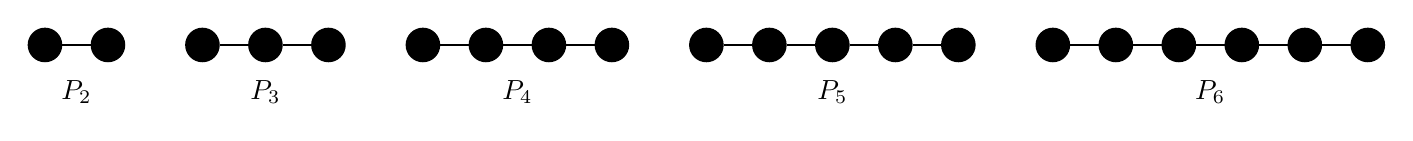
\begin{tikzpicture}[scale=.4]
      \GraphInit[vstyle=Simple]

      \begin{scope}
        \grPath[RA=2]{2}
        \draw (1,-1.5) node {$P_{2}$};
      \end{scope}

      \begin{scope}[xshift=5cm]
        \grPath[RA=2]{3}
        \draw (2,-1.5) node {$P_{3}$};
      \end{scope}

      \begin{scope}[xshift=12cm]
        \grPath[RA=2]{4}
        \draw (3,-1.5) node {$P_{4}$};
      \end{scope}

      %% \begin{scope}[yshift=-3cm]
      \begin{scope}[xshift=21cm]
        \grPath[RA=2]{5}
        \draw (4,-1.5) node {$P_{5}$};
      \end{scope}

      %% \begin{scope}[yshift=-3cm,xshift=10cm]
      \begin{scope}[xshift=32cm]
        \grPath[RA=2]{6}
        \draw (5,-1.5) node {$P_{6}$};
      \end{scope}
    \end{tikzpicture}
  \end{figure*}

  \begin{align*}
    V(P_{v})        &= \Set{ 1, 2, ..., v } \\
    E(P_{v})        &= \Set{ \Set{n-1,n} \colon n \in \Set{ 2, ..., v } } \\
    \abs*{E(P_{v})} &= v - 1 \\
    e               &= v - 1
  \end{align*}
  $\hfill\square$

  \marginnote[-6em]{%
    The number of edges in a \gls{path graph} $P_{v}$, where $v \ge 2$, is
    given by the formula $e = v - 1$.%
  }
  \pagebreak

\item The first five \glspl{wheel graph}.
  \begin{figure*}
    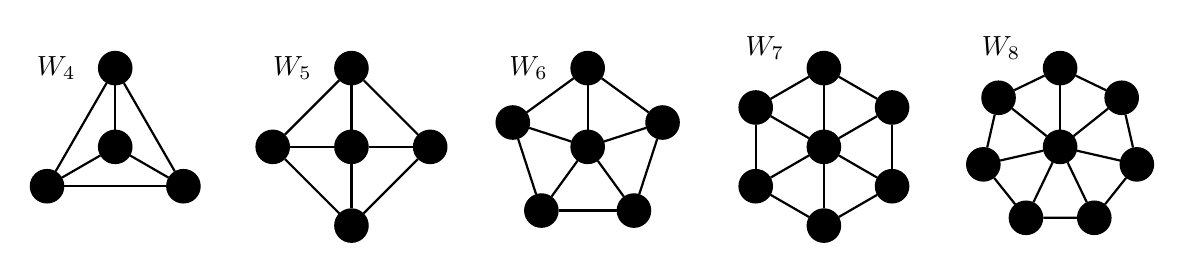
\begin{tikzpicture}[scale=.5]
      \GraphInit[vstyle=Simple]

      \begin{scope}[rotate=90]
        \grWheel[RA=2]{4}
        \draw (2,1.5) node {$W_{4}$};
      \end{scope}

      \begin{scope}[xshift=6cm]
        \grWheel[RA=2]{5}
        \draw (-1.5,2) node {$W_{5}$};
      \end{scope}

      \begin{scope}[xshift=12cm,rotate=90]
        \grWheel[RA=2]{6}
        \draw (2,1.5) node {$W_{6}$};
      \end{scope}

      %% \begin{scope}[xshift=3cm,yshift=-6cm,rotate=90]
      \begin{scope}[xshift=18cm,rotate=90]
        \grWheel[RA=2]{7}
        \draw (2.5,1.5) node {$W_{7}$};
      \end{scope}

      %% \begin{scope}[xshift=9cm,yshift=-6cm,rotate=90]
      \begin{scope}[xshift=24cm,rotate=90]
        \grWheel[RA=2]{8}
        \draw (2.5,1.5) node {$W_{8}$};
      \end{scope}
    \end{tikzpicture}
  \end{figure*}

  \begin{equation*}
    \begin{split}
      V(W_{v})        &= \Set{ 1, 2, 3, ..., v } \\
      E(W_{v})        &= \{\ \Set{1,2}, \Set{1,3}, ..., \Set{1,v}, \\
                      & \qquad \Set{2,3}, \Set{3,4}, ..., \Set{v-1,v}, \\
                      & \qquad \Set{v,2}\ \} \\
                      &= \{\ \Set{ \Set{1,n} \colon n \in \Set{2,...,v} }, \\
                      & \qquad \Set{ \Set{n-1,n} \colon n \in \Set{3,...,v} }, \\
                      & \qquad \Set{v,2}\ \} \\
      \abs*{E(W_{v})} &= (v-1) + (v-2) + 1 \\
                      & = (v-1) + (v-1) \\
      e               & = 2(v-1)
    \end{split}
  \end{equation*}
  $\hfill\square$

  \marginnote[-11em]{%
    The number of edges in the \gls{wheel graph} on $v$ vertices $W_{v}$,
  where $v \ge 4$, is given by the formula $e = 2(v - 1)$.%
  }

\item
  \begin{align*}
    1 + 2 + ... + (v-1) &= (1/2)v(v-1) \\
    &= E(K_{v}) & \text{(T2)} \\
    &= (v-1) + (v-2) + ... + (v - (v-1)) \\
    &= 1 + 2 + ... (v-1)
  \end{align*}
  $\hfill\square$

  \marginnote[-7em]{%
    Imagine drawing $K_{v}$ by joining vertex $1$ to vertices $2$ through $v$,
    creating $v-1$ edges; then joining vertex $2$ to vertices $3$ through $v$,
    creating $v-2$ edges; and so on, i.e.
    $(v - 1) + (v - 2) + ... + (v - (v - 1))$, or equivalently,
    $1 + 2 + ... + (v - 1)$.%
  }

  \item Let $G$ be a graph with $v$ vertices and $e$ edges. In terms of $v$ and
    $e$, $\overline{G}$ has $(1/2)v(v-1) - e$ edges.

    \newpage

  \item \label{ex:9} If a graph $G$ has $v=6$ then $G$ or $\overline{G}$
    (possibly both) has a subgraph isomorphic to $K_{3}$.

    In the graph $G$ or $\overline{G}$ there exists a vertex $a$ of degree three
    or more. Let there be three adjacent vertices $b$, $c$, and $d$. If any of
    the edges $\Set{b,c}$, $\Set{b,d}$, or $\Set{c,d}$ are present in the graph,
    then the graph contains a subgraph isomorphic to $K_{3}$. If none of those
    edges is present, then they are all present in the other graph, which thus
    contains a subgraph isomorphic to $K_{3}$.

    \begin{figure}
      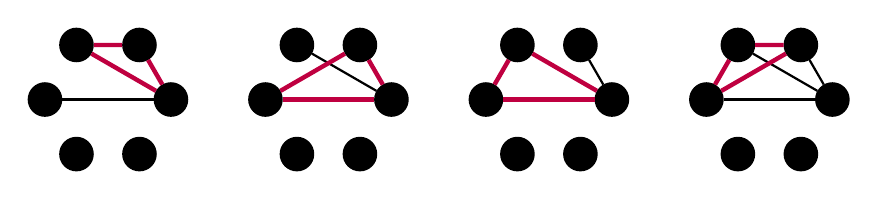
\begin{tikzpicture}[scale=.8]
        \GraphInit[vstyle=Simple]
        \begin{scope}
          \Vertices{circle}{a,b,c,d,e,f}
          \Edge(a)(d)
          \SetUpEdge[color=purple,style={ultra thick}]
          \Edge(a)(b) \Edge(a)(c) \Edge(b)(c)
        \end{scope}

        \begin{scope}[xshift=3.5cm]
          \Vertices{circle}{a,b,c,d,e,f}
          \Edge(a)(c)
          \SetUpEdge[color=purple,style={ultra thick}]
          \Edge(a)(b) \Edge(a)(d) \Edge(b)(d)
        \end{scope}

        \begin{scope}[xshift=7cm]
          \Vertices{circle}{a,b,c,d,e,f}
          \Edge(a)(b)
          \SetUpEdge[color=purple,style={ultra thick}]
          \Edge(a)(c) \Edge(a)(d) \Edge(c)(d)
        \end{scope}

        \begin{scope}[xshift=10.5cm]
          \Vertices{circle}{a,b,c,d,e,f}
          \Edge(a)(b) \Edge(a)(c) \Edge(a)(d)
          \SetUpEdge[color=purple,style={ultra thick}]
          \Edge(b)(c) \Edge(b)(d) \Edge(c)(d)
        \end{scope}
      \end{tikzpicture}
    \end{figure}

    \item From the proof in \hyperref[ex:9]{Exercise~\ref{ex:9}}, it follows
      that in any graph of degree $6$ there exists a subgraph $H$, such that
      either $H$ or $\overline{H}$ is isomorphic to $K_{3}$. Equivalently, in
      any gathering of six people (a graph $G$ with $v=6$) there are either
      three people who are mutually acquainted (a subgraph isomorphic to
      $K_{3}$) or three people who are mutually unacquainted (a subgraph whose
      complement is isomorphic to $K_{3}$).

    \item
      \begin{align}
        2\abs{\emptyset} &= \sum_{v \in V} deg(v) = 0 \tag{BC} \\
        G(V,E) \to 2\abs{E} &= \sum_{v \in V} deg(v) \tag{IH} \\
        H(V^{\prime}, E^{\prime}), \abs{E^{\prime}} &= \abs{E} + 1 \\
        \exists\ H_{0}(V^{\prime}, E^{\prime}_{0}), \abs{E^{\prime}_{0}} &= \abs{E} \\
        2\abs{E^{\prime}_{0}} &= \sum_{v \in V^{\prime}} deg(v) \tag{by IH}\\
        H &\cong (V^{\prime}, E_{0}^{\prime} \cup \Set{e}), e \not\in E_{0}^{\prime} \\
        \sum_{v \in V^{\prime}} deg(v) + 2 &= 2\abs{E} \\
        2\abs{E} + 2 = 2(\abs{E} + 1) &= \sum_{v \in V^{\prime}} deg(v)
      \end{align}
      $\hfill\square$

    \item
      \begin{enumerate}[a)]
      \item
        \begin{align*}
          (4 \times 3) + (2 \times 5) + (2 \times 6) + (1 \times 8) &= 2e \\
          12 + 10 + 12 + 8 &= 2e \\
          21 &= e
        \end{align*}
      \item $(7 \times 3) = 2e \to e \not\in \mathbb{Q}$
      \end{enumerate}
    \item
      \begin{marginfigure}
        \begin{align*}
          n + n &= \frac{n(n-1)}{2} \\
          2n &= \frac{n(n - 1)}{2} \\
          4n &= n(n-1) \\
          4n &= n^{2} - n \\
          0 &= n^{2} - 5n \\
          n &= \Set{0,5}
        \end{align*}
      \end{marginfigure}

      If $C_{n} \cong \overline{C_{n}}$, then it must be the case that \\
      $\abs*{E(C_{n})} + \abs*{E(\overline{C_{n}})} = \abs*{E(K_{n})}$, i.e.
      $n + n = \frac{n(n-1)}{2}$.

      \vskip 1em
      Since $n=5$ is a solution,
      $\abs*{E(C_{5})} + \abs*{E(\overline{C_{5}})} = \abs*{E(K_{5})}$, and thus
      $C_{5} \cong \overline{C_{5}}$. \\
      $\hfill\square$

      \vskip 1em
      A graph with no edges ($n=0$) has no cycles.
      Therefore the only self-complementary cycle graph is $C_{5}$. \\
      $\hfill\square$

    \item If $G \cong \overline{G}$ for a graph $G$ of order $v$, then
      $\abs*{E(G)} + \abs*{E(\overline{G})} = \abs*{E(K_{v})}$, i.e.
      $e + e = 2e = \frac{v(v-1)}{2}$. So the number of edges $e$ in $G$ is
      $\frac{v(v-1)}{4}$, and $4 \mid v(v-1)$. Therefore, for any
      self-complementary graph $G$ of order $v$, $4 \mid v$ or $4 \mid v - 1$.\\
      $\hfill\square$

    \item \todo[color=languidlavender]{Find two other self-complementary graphs
      (Trudeau, \textit{Graph Theory} 57).}

    \item \todo[color=languidlavender]{Find a self-complementary graph with
      $v=8$.}

    \item $P_{4}$ is the self-complementary graph with $v=4$.

    \item Between the two set of $10$ elements, $\Set{a,b,...,j}$ and
      $\Set{1,2,...,10}$, there exist $10!$, or $3,628,800$, one-to-one
      correspondences.

    \item $f: \mathbb{Z}^{+} \to 2\mathbb{Z}^{+}$, $f(x) = 2n$ is bijective.

    \item The first graph in Figure 35 contains a subgraph

      \begin{figure}
        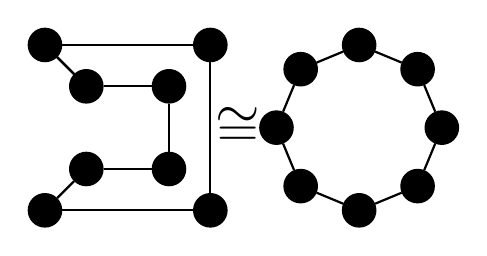
\begin{tikzpicture}[scale=.7]
          \GraphInit[vstyle=Simple]
          \begin{scope}
            \Vertex[x=-1.5,y=1.5]{A}
            \Vertex[x=1.5,y=1.5]{B}
            \Vertex[x=1.5,y=-1.5]{H}
            \Vertex[x=-1.5,y=-1.5]{G}
            \Vertex[x=-.75,y=-.75]{E}
            \Vertex[x=.75,y=-.75]{F}
            \Vertex[x=.75,y=.75]{D}
            \Vertex[x=-.75,y=.75]{C}
            \Edges(C,A,B,H,G,E,F,D,C,A)
          \end{scope}
          \draw (2,0) node {${\huge \cong}$};
          \begin{scope}[xshift=4.2cm]
            \grCycle[RA=1.5]{8}
          \end{scope}
        \end{tikzpicture}
      \end{figure}

      which is isomorphic to $C_{8}$, whereas the second graph contains no
      subgraph isomorphic to $C_{8}$. Therefore, the two graphs are not
      isomorphic.

      \newpage

    \item The 17 unequal subgraphs of $K_{3}$:
      \begin{figure*}
        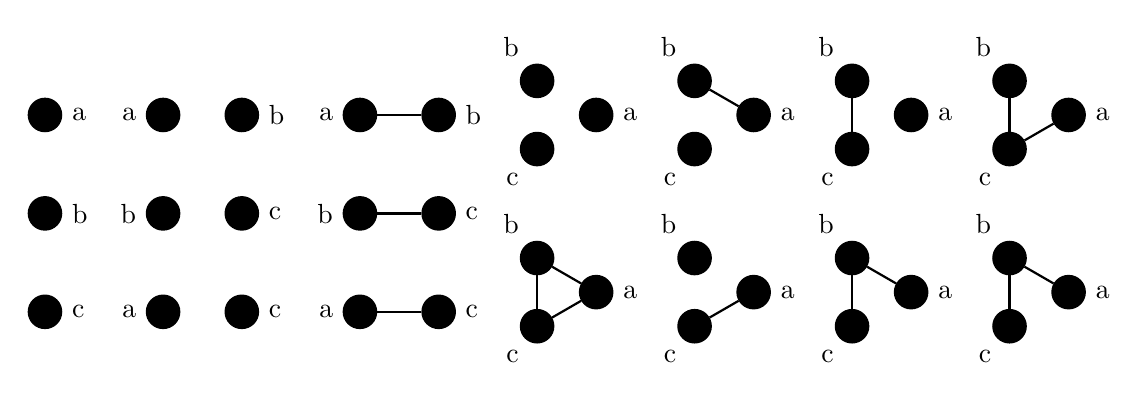
\begin{tikzpicture}[scale=.5]
          \GraphInit[vstyle=Classic]
          \begin{scope}\Vertex{a}\end{scope}
          \begin{scope}[yshift=-2.5cm]\Vertex{b}\end{scope}
          \begin{scope}[yshift=-5cm]\Vertex{c}\end{scope}

          \begin{scope}[xshift=4cm]\Vertices{circle}{b,a}\end{scope}
          \begin{scope}[xshift=4cm,yshift=-2.5cm]\Vertices{circle}{c,b}\end{scope}
          \begin{scope}[xshift=4cm,yshift=-5cm]\Vertices{circle}{c,a}\end{scope}

          \begin{scope}[xshift=9cm]\Vertices{circle}{b,a}\Edges(b,a)\end{scope}
          \begin{scope}[xshift=9cm,yshift=-2.5cm]\Vertices{circle}{c,b}\Edges(c,b)\end{scope}
          \begin{scope}[xshift=9cm,yshift=-5cm]\Vertices{circle}{c,a}\Edges(c,a)\end{scope}

          \begin{scope}[xshift=13cm]\Vertices{circle}{a,b,c}\end{scope}
          \begin{scope}[xshift=13cm,yshift=-4.5cm]\Vertices{circle}{a,b,c}\Edges(a,b,c,a)\end{scope}

          \begin{scope}[xshift=17cm]\Vertices{circle}{a,b,c}\Edges(a,b)\end{scope}
          \begin{scope}[xshift=17cm,yshift=-4.5cm]\Vertices{circle}{a,b,c}\Edges(a,c)\end{scope}

          \begin{scope}[xshift=21cm]\Vertices{circle}{a,b,c}\Edges(b,c)\end{scope}
          \begin{scope}[xshift=21cm,yshift=-4.5cm]\Vertices{circle}{a,b,c}\Edges(a,b,c)\end{scope}

          \begin{scope}[xshift=25cm]\Vertices{circle}{a,b,c}\Edges(b,c,a)\end{scope}
          \begin{scope}[xshift=25cm,yshift=-4.5cm]\Vertices{circle}{a,b,c}\Edges(c,b,a)\end{scope}

        \end{tikzpicture}
      \end{figure*}

    \item The seven nonisomorphic subgraphs of $K_{3}$:
      \begin{figure}
        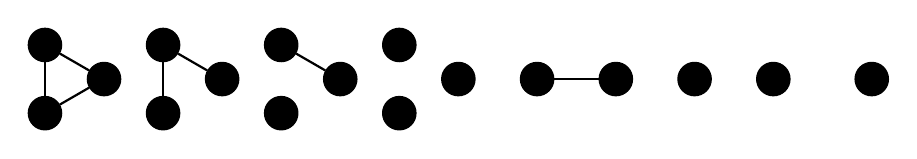
\begin{tikzpicture}[scale=.5]
          \GraphInit[vstyle=Simple]
          \begin{scope}
            \grComplete[RA=1]{3}
          \end{scope}
          \begin{scope}[xshift=3cm]
            \Vertices{circle}{a,b,c}
            \Edges(a,b,c)
          \end{scope}
          \begin{scope}[xshift=6cm]
            \Vertices{circle}{a,b,c}
            \Edges(a,b)
          \end{scope}
          \begin{scope}[xshift=9cm]
            \Vertices{circle}{a,b,c}
          \end{scope}
          \begin{scope}[xshift=13cm]
            \Vertices{circle}{a,b}
            \Edges(a,b)
          \end{scope}
          \begin{scope}[xshift=17cm]
            \Vertices{circle}{a,b}
          \end{scope}
          \begin{scope}[xshift=20.5cm]
            \Vertex{a}
          \end{scope}
        \end{tikzpicture}
      \end{figure}

    \item $C_{3}$ is a subgraph of the first graph, but not the
      second. Therefore, the two graphs are not isomorphic.

    \item The graphs of Figure 31 are not isomorphic because their complements
      have different degree distributions: the first has one vertex of degree 2,
      two of degree 1, and four of degree 0, whereas the second has four of
      degree 1, and three of degree 0.
      \begin{marginfigure}[-5em]
        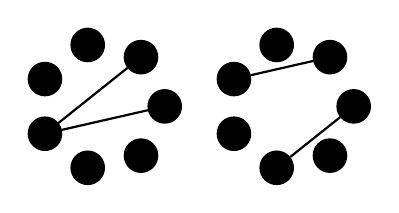
\begin{tikzpicture}[scale=.8]
          \GraphInit[vstyle=Simple]
          \begin{scope}
            \grEmptyCycle[RA=1,prefix=]{7}
            \Edges(0,4)
            \Edges(1,4)
          \end{scope}
          \begin{scope}[xshift=3cm]
            \grEmptyCycle[RA=1,prefix=]{7}
            \Edges(0,5)
            \Edges(1,3)
          \end{scope}
        \end{tikzpicture}
      \end{marginfigure}

    \item The graphs of Figure 46 are not isomorphic beacuse their complements
      are nonisomorphic, as shown below. Notably, the cyan edges in one
      complement are missing in the other.
      \begin{figure}
        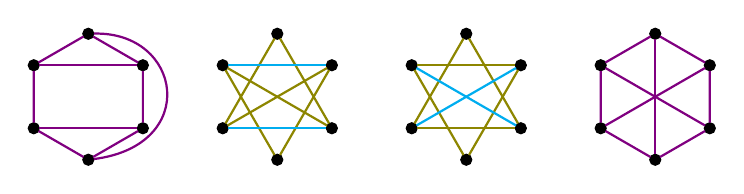
\begin{tikzpicture}[scale=.8]
          \SetVertexSimple
          \SetGraphUnit{1}
          \tikzset{VertexStyle/.style = {
              shape = circle,
              fill = black,
              inner sep = 0pt,
              outer sep = 0pt,
              minimum size = 4pt,
              draw}}
          \begin{scope}[rotate=90]
            \grEmptyCycle[RA=1,prefix=]{6}
            \tikzstyle{EdgeStyle}=[color=violet]
            \Edge[style={out=-85, in=-80, out looseness=1.9, in looseness=2.3}](0)(3)
            \Edge(0)(1)
            \Edge(0)(5)
            \Edge(1)(2)
            \Edge(1)(5)
            \Edge(2)(3)
            \Edge(2)(4)
            \Edge(3)(4)
            \Edge(4)(5)
          \end{scope}
          \begin{scope}[xshift=3cm,rotate=90]
            \grEmptyCycle[RA=1,prefix=]{6}
            \SetUpEdge[style={color=olive}]
            \Edge(0)(2)
            \Edge(0)(4)
            \Edge(1)(3)
            \Edge(1)(4)
            \Edge(2)(5)
            \Edge(3)(5)
            \tikzstyle{EdgeStyle}=[color=cyan]
            \Edge(1)(5)
            \Edge(2)(4)
          \end{scope}
          \begin{scope}[xshift=6cm,rotate=90]
            \grEmptyCycle[RA=1,prefix=]{6}
            \tikzstyle{EdgeStyle}=[color=olive]
            \Edge(0)(2)
            \Edge(0)(4)
            \Edge(1)(3)
            \Edge(1)(5)
            \Edge(2)(4)
            \Edge(3)(5)
            \tikzstyle{EdgeStyle}=[color=cyan]
            \Edge(1)(4)
            \Edge(2)(5)
          \end{scope}
          \begin{scope}[xshift=9cm,rotate=90]
            \grEmptyCycle[RA=1,prefix=]{6}
            \tikzstyle{EdgeStyle}=[color=violet]
            \Edge(0)(1)
            \Edge(0)(3)
            \Edge(0)(5)
            \Edge(1)(2)
            \Edge(1)(4)
            \Edge(2)(3)
            \Edge(2)(5)
            \Edge(3)(4)
            \Edge(4)(5)
          \end{scope}
        \end{tikzpicture}
      \end{figure}

      \newpage
    \item Drawn below are all 34 graphs having $v=5$.
      \begin{figure*}
        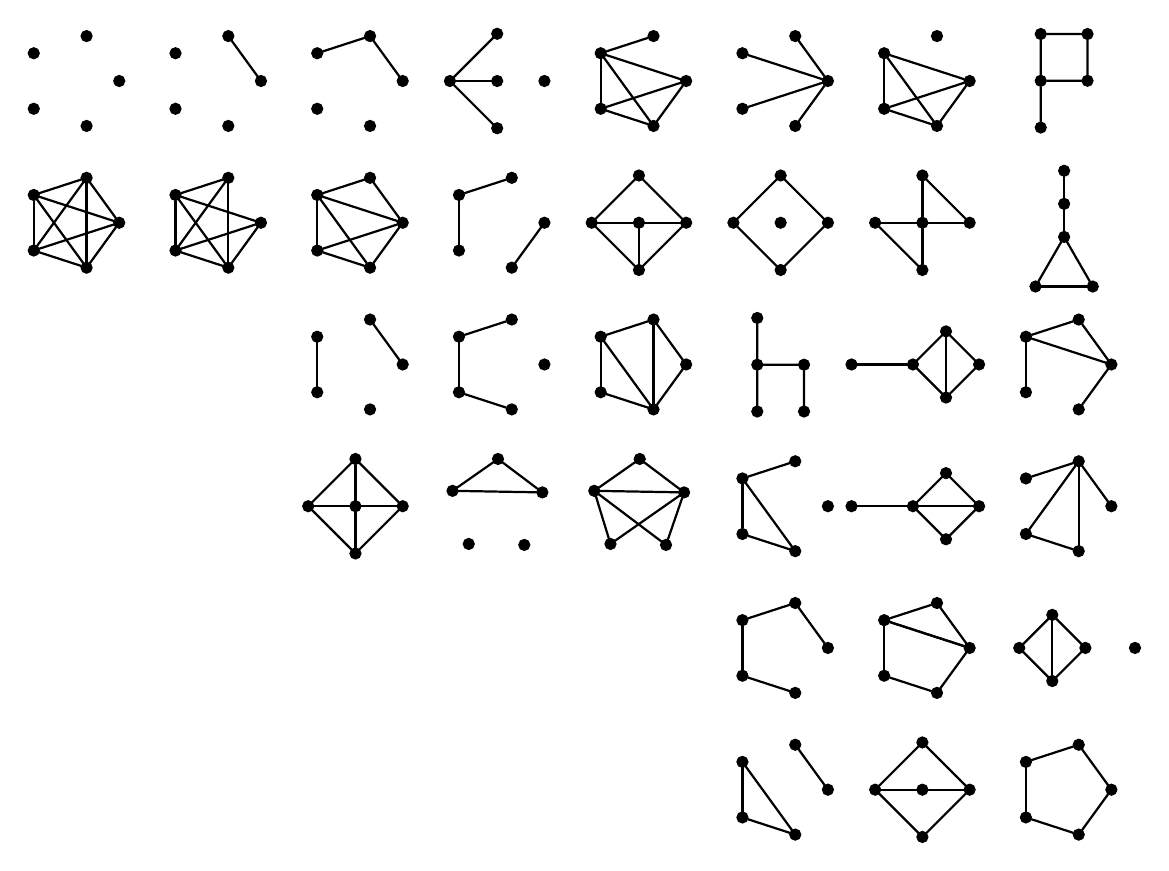
\begin{tikzpicture}[scale=.6]
          \SetVertexSimple
          %% \GraphInit[vstyle=Classic]
          \SetGraphUnit{1}
          \tikzset{VertexStyle/.style = {
              shape = circle,
              fill = black,
              inner sep = 0pt,
              outer sep = 0pt,
              minimum size = 4pt,
              draw}}
          \begin{scope}
            \grEmptyCycle[RA=1,prefix=]{5}
          \end{scope}
          \begin{scope}[yshift=-3cm]
            \grComplete[RA=1,prefix=]{5}
          \end{scope}
          \begin{scope}[xshift=3cm]
            \grEmptyCycle[RA=1,prefix=]{5}
            \Edge(0)(1)
          \end{scope}
          \begin{scope}[xshift=3cm,yshift=-3cm]
            \grEmptyCycle[RA=1,prefix=]{5}
            \Edges(1,2,3,4,0)
            \Edges(1,4,2,0,3,1)
          \end{scope}
          \begin{scope}[xshift=6cm]
            \grEmptyCycle[RA=1,prefix=]{5}
            \Edges(0,1,2)
          \end{scope}
          \begin{scope}[xshift=6cm,yshift=-3cm]
            \grEmptyCycle[RA=1,prefix=]{5}
            \Edges(0,2,3,4,0)
            \Edges(4,2,1,0,3)
          \end{scope}
          \begin{scope}[xshift=6cm,yshift=-6cm]
            \grEmptyCycle[RA=1,prefix=]{5}
            \Edge(0)(1)
            \Edge(2)(3)
          \end{scope}
          \begin{scope}[xshift=6cm,yshift=-9cm]
            \grWheel[RA=1,prefix=]{5}
          \end{scope}
          \begin{scope}[xshift=9cm]
            \grEmptyStar[RA=1,prefix=]{5}
            \Edges(1,2,3)
            \Edge(2)(4)
          \end{scope}
          \begin{scope}[xshift=9cm,yshift=-3cm]
            \grEmptyCycle[RA=1,prefix=]{5}
            \Edges(1,2,3)
            \Edge(0)(4)
          \end{scope}
          \begin{scope}[xshift=9cm,yshift=-6cm]
            \grEmptyCycle[RA=1,prefix=]{5}
            \Edges(1,2,3,4)
          \end{scope}
          \begin{scope}[xshift=9cm,yshift=-9cm,rotate=-55]
            \grEmptyCycle[RA=1,prefix=]{5}
            \Edges(1,2,3,1)
          \end{scope}
          \begin{scope}[xshift=12cm]
            \grEmptyCycle[RA=1,prefix=]{5}
            \Edges(1,2,3,4,0)
            \Edges(4,2,0,3)
          \end{scope}
          \begin{scope}[xshift=12cm,yshift=-3cm]
            \grEmptyStar[RA=1,prefix=]{5}
            \Edges(0,1,2)
            \Edges(3,4,0,3,2,4)
          \end{scope}
          \begin{scope}[xshift=12cm,yshift=-6cm]
            \grEmptyCycle[RA=1,prefix=]{5}
            \Edges(0,1,2,3,4,0)
            \Edges(2,4,1)
          \end{scope}
          \begin{scope}[xshift=12cm,yshift=-9cm,rotate=-55]
            \grEmptyCycle[RA=1,prefix=]{5}
            \Edges(1,2,3,1,4,3,0,1)
          \end{scope}query
          \begin{scope}[xshift=15cm]
            \grEmptyCycle[RA=1,prefix=]{5}
            \foreach \v in {1,2,3,4}{\Edge(0)(\v)};
          \end{scope}
          \begin{scope}[xshift=15cm,yshift=-3cm]
            \grEmptyStar[RA=1,prefix=]{5}
            \Edges(0,1,2,3,0)
          \end{scope}
          \begin{scope}[xshift=15cm,yshift=-6.5cm,rotate=45]
            \grEmptyCycle[RA=.7,prefix=]{4}
            \Edges(3,0,1,2)
            \Vertex[x=.7,y=1.4]{4}
            \Edge(4)(1)
          \end{scope}
          \begin{scope}[xshift=15cm,yshift=-9cm]
            \grEmptyCycle[RA=1,prefix=]{5}
            \Edges(2,3,4,2)
            \Edge(2)(1)
          \end{scope}
          \begin{scope}[xshift=15cm,yshift=-12cm]
            %% \grPath[RA=1,prefix=]{5}
            \grEmptyCycle[RA=1,prefix=]{5}
            \Edges(0,1,2,3,4)
          \end{scope}
          \begin{scope}[xshift=15cm,yshift=-15cm]
            \grEmptyCycle[RA=1,prefix=]{5}
            \Edges(2,3,4,2)
            \Edge(0)(1)
          \end{scope}
          \begin{scope}[xshift=18cm]
            \grEmptyCycle[RA=1,prefix=]{5}
            \Edges(3,0,4,2)
            \Edges(0,2,3,4)
          \end{scope}
          \begin{scope}[xshift=18cm,yshift=-3cm]
            \grEmptyStar[RA=1,prefix=]{5}
            \Edges(0,1,4,2,3,4,0)
          \end{scope}
          \begin{scope}[xshift=18.5cm,yshift=-6cm]
            \grCycle[RA=.7,prefix=]{4}
            \Vertex[x=-2,y=0]{4}
            \Edge(1)(3)
            \Edge(4)(2)
          \end{scope}
          \begin{scope}[xshift=18.5cm,yshift=-9cm]
            \grCycle[RA=.7,prefix=]{4}
            \Vertex[x=-2,y=0]{4}
            \Edges(4,2,0)
          \end{scope}
          \begin{scope}[xshift=18cm,yshift=-12cm]
            \grEmptyCycle[RA=1,prefix=]{5}
            \Edges(0,2,1,0,4,3,2,0)
          \end{scope}
          \begin{scope}[xshift=18cm,yshift=-15cm]
            \grEmptyStar[RA=1,prefix=]{5}
            \Edges(0,1,2,3,0,4,2)
          \end{scope}
          \begin{scope}[xshift=21cm,yshift=.5cm,rotate=225]
            \grEmptyCycle[RA=.7,prefix=]{4}
            \Vertex[x=1.4,y=.7]{4}
            \Edges(0,1,2,3,0,4)
          \end{scope}
          \begin{scope}[xshift=21cm,yshift=-4cm,rotate=90]
            \grCycle[RA=.7,prefix=]{3}
            \Vertices[dir=\EA,x=1.4,y=0,unit=.7]{line}{3,4}
            \Edges(4,3,0)
          \end{scope}
          \begin{scope}[xshift=21cm,yshift=-6cm]
            \grEmptyCycle[RA=1,prefix=]{5}
            \Edges(1,2,0,1)
            \Edge(2)(3)
            \Edge(0)(4)
          \end{scope}
          \begin{scope}[xshift=21cm,yshift=-9cm]
            \grEmptyCycle[RA=1,prefix=]{5}
            \Edges(0,1,4,3,1,2)
          \end{scope}
          \begin{scope}[xshift=20.75cm,yshift=-12cm,rotate=180]
            \grCycle[RA=.7,prefix=]{4}
            \Vertex[x=-1.75,y=0]{4}
            \Edge(1)(3)
          \end{scope}
          \begin{scope}[xshift=21cm,yshift=-15cm]
            \grCycle[RA=1,prefix=]{5}
          \end{scope}
        \end{tikzpicture}
      \end{figure*}

    \item \todo[color=languidlavender]{There are an odd number of nonisomorphic
      graphs with $v=4$. Is this special? Are there other values of $v$ for
      which the number of nonisomorphic graphs is also odd? (Trudeau, \textit{Graph Theory} 59).
    \url{https://math.stackexchange.com/questions/86790/is-there-a-reason-why-the-number-of-non-isomorphic-graphs-with-v-4-is-odd}}

\end{enumerate}

\backmatter

\phantomsection
\printglossaries

\end{document}
